% Использован шаблон:
% https://www.writelatex.com/coursera/latex/1.1
% http://coursera.org/course/latex


\documentclass[a4paper,12pt]{article}

\usepackage{cmap}
\usepackage[T2A]{fontenc}
\usepackage[utf8]{inputenc}
\usepackage[english,russian]{babel}
\usepackage{fancyhdr}
\usepackage{minted}
\usepackage{hyperref}
\usepackage{amsmath}
\usepackage{graphicx}
\usepackage{xcolor}

\hypersetup{
  pdfborderstyle={/S/U/W 1}
}

\graphicspath{{./images/}}

\pagestyle{fancy}
\fancyhf{}
\lhead{Антон Завьялов, ПИ-72}
\rhead{\textbf{Лабораторная №7. Вариант 1}}
\cfoot{\thepage}

\makeatletter
\def\@seccntformat#1{%
  \expandafter\ifx\csname c@#1\endcsname\c@section\else
  \csname the#1\endcsname\quad
  \fi}
\makeatother

\begin{document} % Конец преамбулы, начало текста.

\begin{center}
  \textbf{Лабораторная работа №7 по дисциплине\linebreak"Компьютерная графика"\linebreak\linebreakВыполнил студент группы ПИ-72 Завьялов А.А.}\\
\end{center}

\section{\normalsize{Задание}}
\begin{flushleft}
Для произвольного изображения выполнить масштабирование с произвольным коэффициентом. В качестве тестовых изображении взять:

\begin{itemize}
    \item Изображение с фотокачеством
    \item Произвольные геометрические фигуры (кольца, круги, линии).
\end{itemize}

Выполнить сглаживание и провести сравнительный анализ следующих методов:

\textbf{1 вариант}

\begin{itemize}
    \item Ближайшего соседа
    \item Билинейное сглаживание
\end{itemize}

\end{flushleft}

\section{\normalsize{Исходный код}}
Исходный код программы также расположен в Git-репозитории по адресу: \url{https://github.com/andiogenes/cg/tree/master/image-processing}
\inputminted[breaklines]{py}{../resampling.py}

\section{\normalsize{Скриншоты, демонстрирующие работу программы}}
\begin{flushleft}
  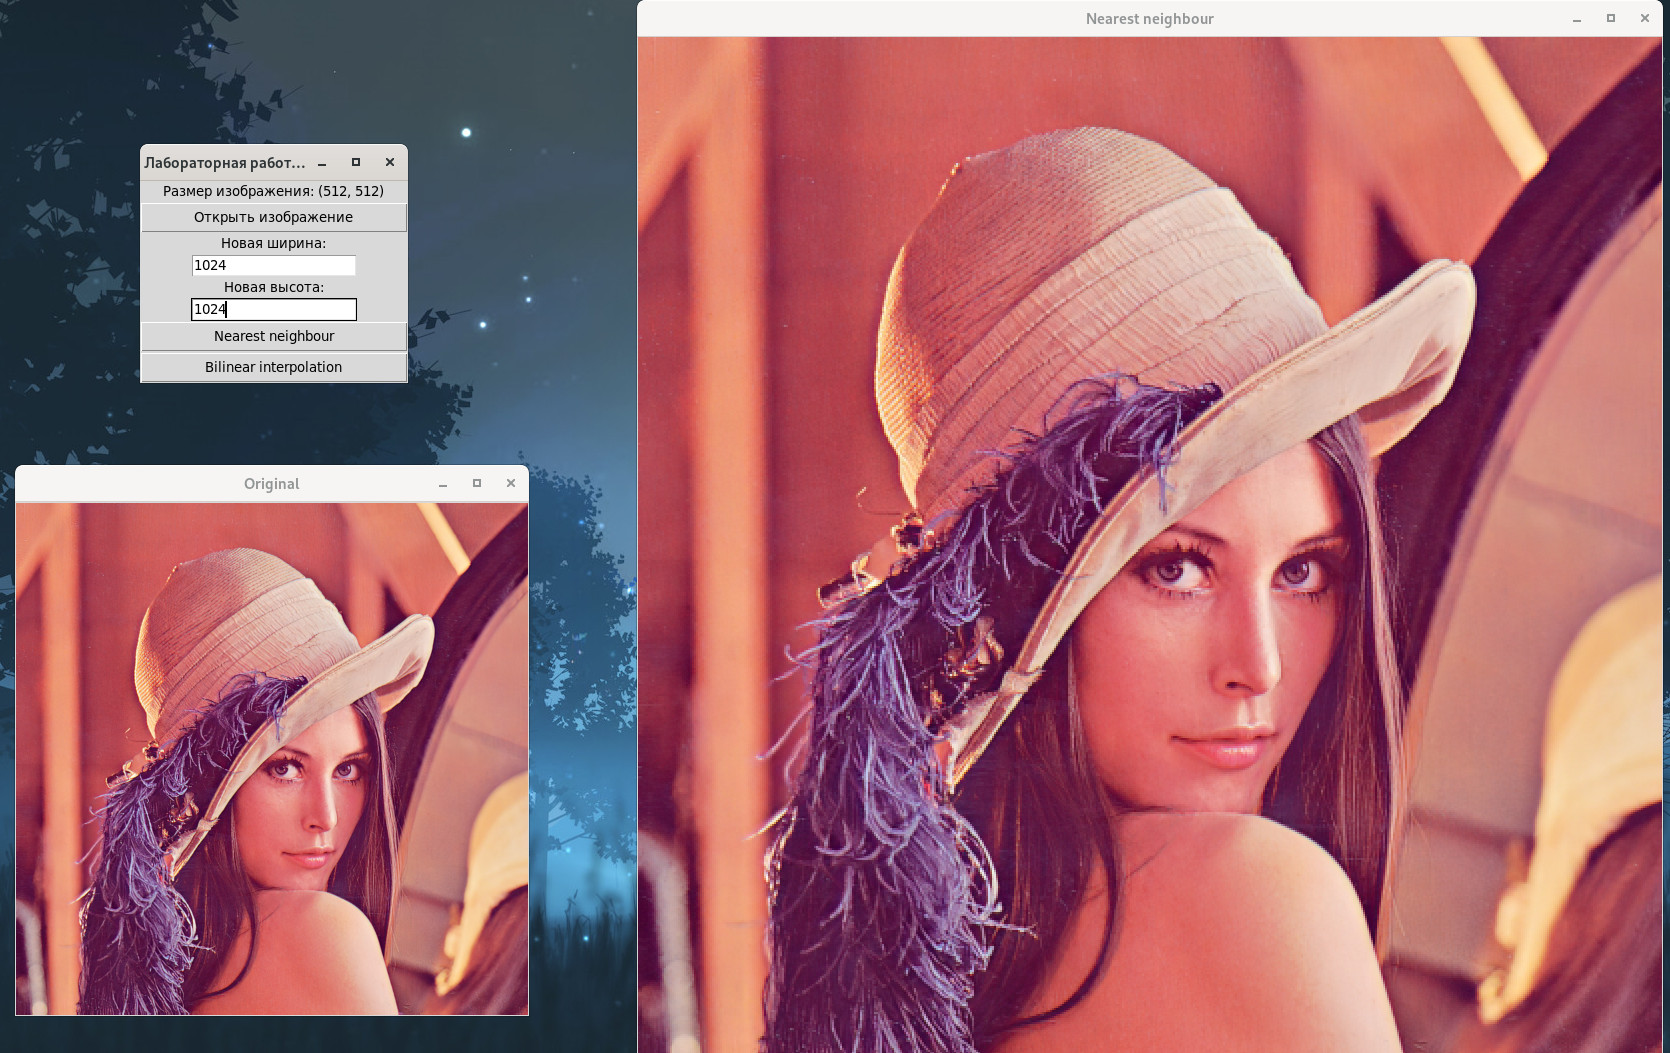
\includegraphics[scale=1]{nearest_1.jpg}
  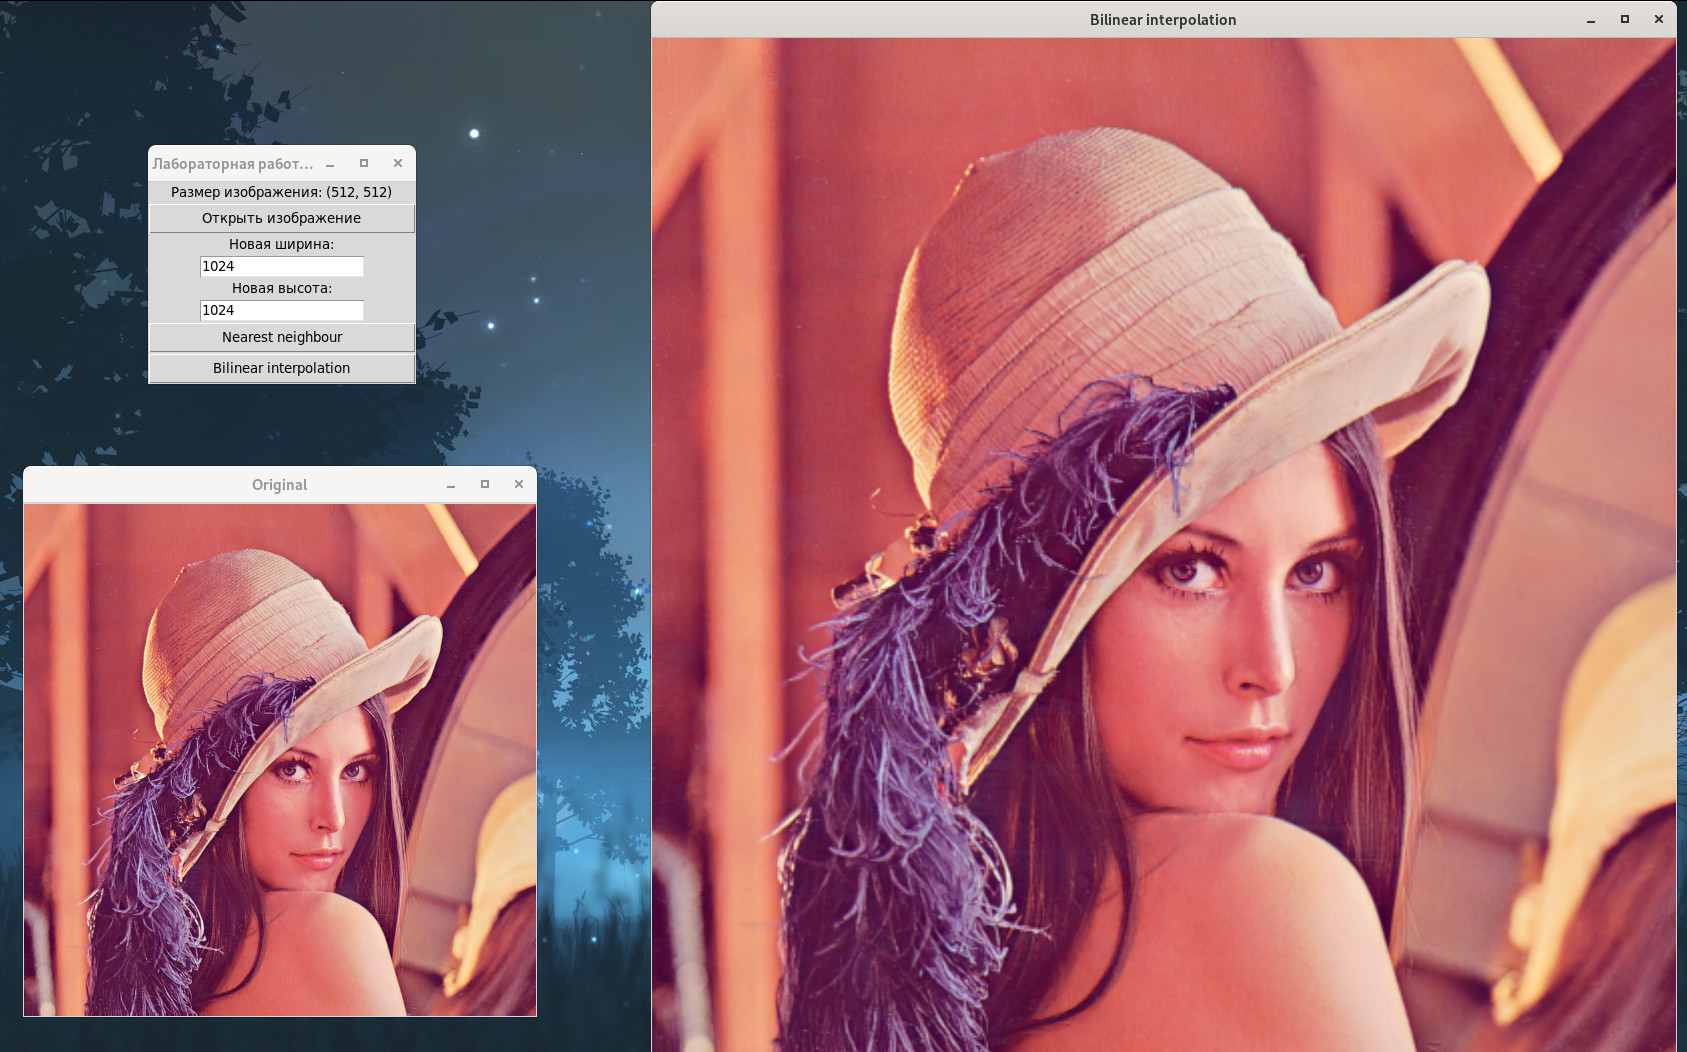
\includegraphics[scale=1]{bilinear_1.jpg}
  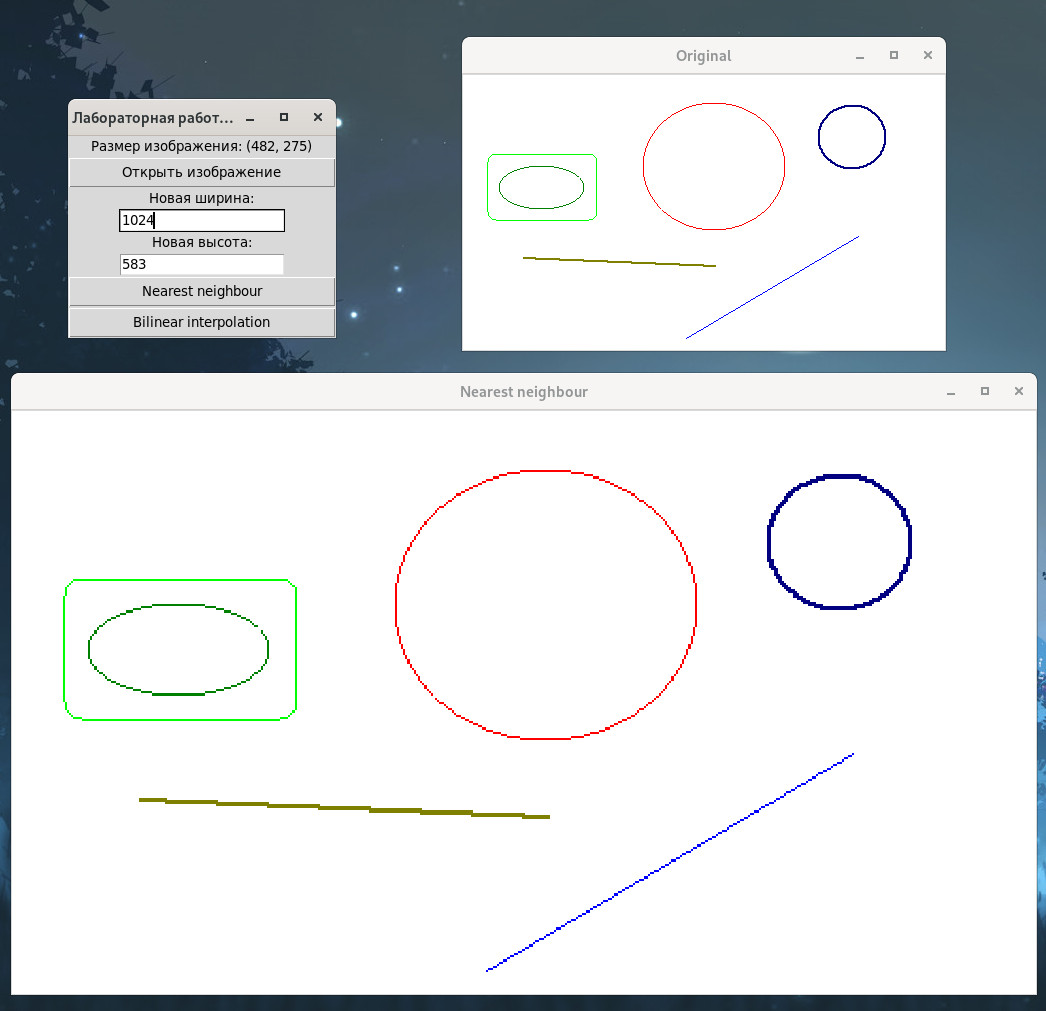
\includegraphics[scale=1.5]{nearest_2.jpg}
  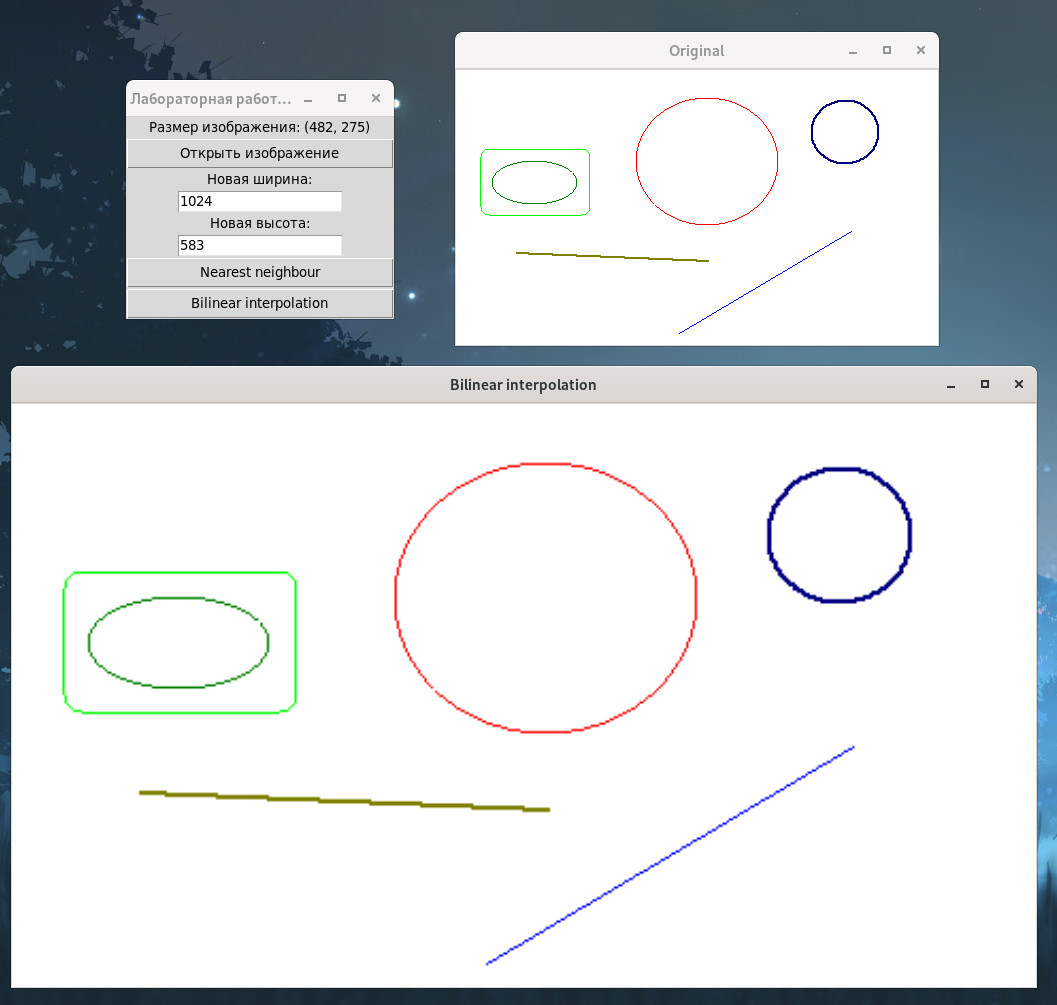
\includegraphics[scale=1.5]{bilinear_2.jpg}
\end{flushleft}

\begin{flushleft}
  По полученным изображениям видно, что для комплексных изображений, в частности, фотографий, качественнее масштабирует алгоритм билинейной интерполяции; изображения, с ''острыми углами'', для которых требуется попиксельная точность (pixel-perfect) -  метод ближайшего соседа.
\end{flushleft}
\end{document}

